\documentclass[conference]{IEEEtran}
%\IEEEoverridecommandlockouts
% The preceding line is only needed to identify funding in the first footnote. If that is unneeded, please comment it out.
\usepackage{cite}
\usepackage{amsmath,amssymb,amsfonts}
\usepackage{algorithmic}
\usepackage{graphicx}
\usepackage{verbatim}
\usepackage{comment}
\usepackage{tikz}
\usetikzlibrary{shapes,arrows,positioning,calc}
\usepackage{textcomp}
\usepackage{xcolor}
\def\BibTeX{{\rm B\kern-.05em{\sc i\kern-.025em b}\kern-.08em
    T\kern-.1667em\lower.7ex\hbox{E}\kern-.125emX}}
\tikzset{
        block/.style = {draw, fill=white, rectangle, minimum height=3em, minimum width=3em},
        input/.style = {coordinate,node distance=1cm},
        output/.style = {coordinate,node distance=4cm},
        line/.style={draw, -latex'}}
        
\begin{document}

\title{Implementation of a Machine Learning based OFDM detector using GNU Radio
}

\makeatletter
\newcommand{\linebreakand}{%
  \end{@IEEEauthorhalign}
  \hfill\mbox{}\par
  \mbox{}\hfill\begin{@IEEEauthorhalign}
}
\makeatother
\renewcommand\IEEEkeywordsname{Keywords}

\author{\IEEEauthorblockN{Kaustubh Venkatesh}
\IEEEauthorblockA{\textit{Department of Electronics and Telecommunications} \\
\textit{Sardar Patel Institute of Technology}\\
Mumbai-58, India \\
kaustubh.v@spit.ac.in}
\and
\IEEEauthorblockN{Gokul Nair}
\IEEEauthorblockA{\textit{Department of Electronics and Telecommunications} \\
\textit{Sardar Patel Institute of Technology}\\
Mumbai-58, India \\
gokul.nair@spit.ac.in}
\linebreakand
\IEEEauthorblockN{Sukanya Kulkarni}
\IEEEauthorblockA{\textit{Department of Electronics and Telecommunications} \\
\textit{Sardar Patel Institute of Technology}\\
Mumbai-58, India \\
sukanya\_kulkarni@spit.ac.in}

}

\maketitle

\begin{abstract}
 Software-Defined Radios (SDRs) are powerful and versatile tools that can implement various communication systems in the software domain. The user can redefine the system by modifying the code. GNU Radio is an open-source SDR that uses a block-based graphical interface with a Python backend framework. Machine Learning (ML) technologies are powerful tools that can bolster the development of the next generation of wireless communication systems. Orthogonal frequency-division multiplexing (OFDM) is a modulation scheme used in modern communication systems such as 4G/5G, WiMax, etc. This study uses the powerful ML ecosystem in Python to model conventional OFDM receivers using the GNU Radio ecosystem. The work trains and compares Deep Neural Networks as well as Linear Regression algorithms (using PHY-layer data) to model the receiver. The trained models improve upon the Bit Error Rate (BER) of conventional systems by a factor of 10$^{-2}$.
\end{abstract}


\begin{IEEEkeywords}
SDR, GNU Radio, Machine Learning, OFDM, Deep Neural Networks
\end{IEEEkeywords}

\section{Introduction}

Wireless digital communication has burgeoned since the beginning of the 21st century, allowing millions access to reliable information. The rapid increase in demand calls for better and more efficient methods for system implementation. Modern wireless communication technologies such as 4G/LTE, 5G, and WiMax \cite{b1} utilize Orthogonal frequency-division multiplexing (OFDM) as a modulation scheme. OFDM overcomes frequency-selective fading and improves spectral efficiency in communication channels \cite{b2}.

Traditionally, data is sent through a single channel serially and hence any interference to that particular frequency can disrupt the entire transmission. OFDM is a form of multi-carrier modulation. It utilizes multiple closely spaced sub-carriers that are orthogonal to each other to carry data in parallel. Analysis of an OFDM receiver can help understand the working of the system. The receiver functions as a series of demodulators and converts each carrier into DC. Data is regenerated from the carrier by integrating the resulting signal over the symbol period \cite{b3}.

This study plans to implement an OFDM system using a Software Defined Radio (SDR). An SDR implements conventional hardware-based communication systems using software, allowing the user to modify the system easily. It also allows the system to integrate efficiently with peripheral software tools. GNU Radio is an open-source SDR toolkit that uses a block-based interface to implement signal processing systems. It is also available as a Python library.

The study uses Machine Learning (ML) and Deep Neural Networks (DNN) to refine the results obtained from  GNU Radio. The utilization of computational power of processors aids in achieving higher accuracy and solutions closer to ideal values. 

\section{Related Work}
Current wireless communication standards use OFDM that requires high data rates and low error rates when transmitting over wireless multi-path channels \cite{b1}. A sizable number of studies thus recommend the application of ML in wireless communication technologies. These studies use the fact that DNNs can analyze and remember convoluted characteristics of wireless channels and are hence used for channel estimation \cite{b2} and symbol detection \cite{b4} \cite{b5} in OFDM systems. The latest studies have used linearly activated fully-connected layers \cite{b4} in models.

The use of an SDR for implementing IEEE 802.11a (which uses OFDM)  is studied in \cite{b6}. Some studies on implementing OFDM using GNU Radio \cite{b7} have been conducted, which is a less-explored domain. \cite{b8} also studies OFDM with different modulation techniques and compares the relative Bit Error Rates (BER). While there have been efforts made to integrate DNNs with the GNU Radio environment \cite{b9}, these use external engines and frameworks to implement the proposed algorithms. The creation of real-time, high-quality datasets for ML projects\cite{b10} is possible using GNU Radio.

The main contribution of this study is the identification and utilization of the Python-based back-end framework of the GNU Radio Companion toolkit. The study proposes Python due to its exhaustive ML technology stack that can be used within the GNU Radio framework.

The organization of the paper is as follows. Section III delineates the specifications of the ML models used, their component layers, and features. Section IV defines the steps undertaken to choose and develop the machine learning algorithms and describes the performance metrics. Section V walks through the outcome of the study and explains its significance. Section VI concludes the study and summarizes the benefits of using ML in OFDM systems and how the results correlate with the expected outcome.

\section{Experimental Design}
The GNU Radio Companion (GRC) application uses Python as its back-end to implement the flow-graph created. The application generates a Python script that can be modified to add relevant functionality.

Linear regression algorithms model a system using the data by calculating the coefficients of an approximate analogous linear system. The Python library Scikit-learn contains modules which implement these algorithms.

DNNs are supervised, non-linear models that use many layers of artificial neural networks, weights, biases, and activation functions. The algorithm updates the weights and biases based on the error at every level of training which is known as back-propagation. Back-propagation helps improve the performance of the model. Keras and TensorFlow are Python libraries which implement various DNN algorithms. Fig. 1 shows the construction of the DNN model (based on regression) developed for modelling the receiver. The DNN model uses ReLU as the activation function for its layers. There are three hidden layers. The model consists of 32 neurons or nodes with 317 trainable parameters. The output layer of the DNN model utilizes a linear activation function to achieve regression results. The study implements the ML algorithms to develop detectors which use BPSK and QPSK modulation schemes.

The program uses multi-threading (a feature of Python) to receive and transmit data while training the models and predicting outcomes. Since Python uses C to implement its code, embedded systems and other mobile wireless communication systems can effectively use these models to improve performance.

\begin{figure}[htpb]
\centerline{\includegraphics[scale = 0.38]{model_plot.png}}
\caption{Construction of the DNN model for QPSK}
\label{dnn_model_plot}
\end{figure}

\section{Implementation}
This section details the steps taken to develop and train the chosen Machine Learning algorithms to model the OFDM detector.

\subsection{Experimental Setup}
The study uses GNU Radio 3.8.1 on a Windows PC to implement the OFDM transmitter and receiver pair and simulate transmission through a channel model. The work uses the Anaconda (Spyder) scientific programming environment which includes Pandas, TensorFlow, Keras, Matplotlib, NumPy, and Scikit-learn Python libraries to add the ML features.  


\subsection{Flowgraph and Data Extraction}
 The flow-graph derives its features from the IEEE 802.11a standards \cite{b5} which is available as an example program in the GNU Radio package. The work modifies the flow-graph by adding signal probes at appropriate locations to extract the required data. Fig. 2 shows the flow-graph of the OFDM receiver used. The study modifies the generated Python file to add the algorithm designed to implement the detector. Fig. 3 and 4 show the time and frequency domain representation of the generated OFDM signal respectively. The flow-graph uses pseudo-random 8-bit bytes as the input data to be modulated. The algorithm deploys Python's sleep function to synchronize data extraction at the transmitting and receiving ends.
 
\begin{figure}[htbp]
\centerline{\includegraphics[width=9cm]{tx_ofdm.png}}
\caption{Flow-graph of a typical OFDM receiver}
\label{flowgraph}
\end{figure}

\begin{figure}[htbp]
\centerline{\includegraphics[width=9cm]{waveform.jpg}}
\caption{Time-domain waveform of the received OFDM signal}
\label{waveform}
\end{figure}

\begin{figure}[htbp]
\centerline{\includegraphics[width=9cm]{spectrum.jpg}}
\caption{Frequency spectrum of the received OFDM signal}
\label{spectrum}
\end{figure}

\subsection{Model Training and Deployment}
The model training phase of the algorithm extracts data from the transmission of 100,000 data frames through an ideal channel. The algorithm uses the received signal, decoded data stream, and the output signal (PHY-layer data) as training data \cite{b2}. It then stores the data in a CSV file. The program performs data cleaning and preprocessing (scaling and feature selection) using Pandas. The algorithm then trains the models (DNN and Linear Regression) and measures the required metrics. The program then saves the trained model for later use. Fig. 5 shows the block diagram of the proposed algorithm.


\begin{figure}[htbp]
%\centerline{\includegraphics[scale=0.35]{algoflow.png}}
\centering
    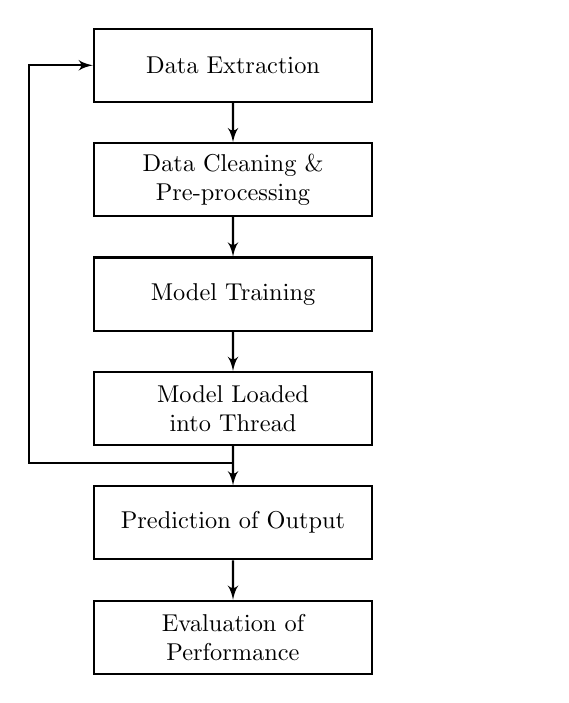
\begin{tikzpicture}[thick,scale=0.82, every node/.style={scale=0.88},text width=25ex, node distance=0.5cm, align=center,>=latex']
            \node [block] (ext) {Data Extraction};
            \node [block, below=of ext] (clean) {Data Cleaning \& Pre-processing};
            \node [block, below=of clean] (train) {Model Training};
            \node [block, below=of train] (load) {Model Loaded into Thread};
            \node [block, below=of load] (pred) {Prediction of Output};
            \node [block, below=of pred] (eval) {Evaluation of Performance};

            \begin{scope}[line]
            \draw (ext) -- (clean);
            \draw (clean) -- (train);
            \draw (train) -- (load);
            \draw (load) -- (pred);
            \draw (load.south) |- ++ (-9em,-0.75em) |- (ext)
            node[pos=4.5,left,align=left]{};
            \draw (pred) -- (eval);
            \end{scope}
    \end{tikzpicture} 
\caption{Flowchart of the Algorithm}
\label{algo}
\end{figure}

\begin{figure}[htbp]
\centerline{\includegraphics[width=7.9cm]{loss_qpsk_v2.png}}
\caption{Plot of MSE (loss) vs Epochs for training the DNN model for QPSK}
\label{loss_qpsk}
\end{figure}

\begin{figure}[htbp]
\centerline{\includegraphics[width=8cm]{mae_qpsk_v2.png}}
\caption{Plot of MAE vs Epochs for training the DNN model for QPSK}
\label{mae_qpsk}
\end{figure}

% Edit plot?
The performance metrics used for the DNN model are Mean Square Error (MSE) and Mean Absolute Error (MAE). Fig. 6 and 7 show the plot of MSE (loss) and MAE during training against the number of epochs respectively for QPSK modulation. The DNN model for QPSK achieves a low MSE of 0.01 and MAE of 0.05 after training it for 30 epochs. The formula for MSE of a DNN model is:
\begin{equation}
     MSE = \displaystyle\frac{1}{n}\sum_{i=1}^{n}(Y_i - X_i)^2
\label{mse}
\end{equation}
where,\\
{n}	=	number of data points,\\
${Y_i}$	=	observed values,\\
${X_i}$	=	predicted values.

The formula for MAE of a DNN model is : 
\begin{equation}
    MAE = \frac{1}{n}\sum_{i=1}^{n}|y_i - x_i|
\end{equation}
where, \\
${y_i}$	=	prediction, \\
${x_i}$	=	true value, \\
{n}	=	total number of data points.\\

The metric used for the linear regression model is R$^{2}$ score. The linear regression model achieves a score of 88.3 \% for QPSK modulation and 93.4 \% for BPSK modulation. The formula for R$^{2}$ score of the linear model is given by : 
\begin{equation}
    R^{2} = {1 - \frac{SS_{res}}{SS_{tot}}}
\end{equation}
where,\\
${SS_{res}}$ = total sum of squares,\\
${SS_{tot}}$ = residual sum of squares.\\


The transmitted signal passes through a simulated channel model to form the received signal. The algorithm then loads the trained model into the multi-threaded program within the GNU Radio environment. The model predicts the expected output based on the received signal from the signal probes. The study implements a decision algorithm to choose the best result from both models. The program then calculates the Bit Error Rate (BER) for the system for different values of Signal-to-noise ratio (SNR). The algorithm uses new data (1500 frames spaced over the runtime) it encounters to retrain the models and improve upon the results. 

\section{Simulation Results}
This section highlights the improved performance of the implemented machine learning-based detector over the conventional receiver system. The study evaluates the detector using BER and plots them against various SNR values.


\begin{figure}[htbp]
\centerline{\includegraphics[width=9cm]{ber_plot_qpskv2.jpg}}
\caption{Comparison of BER plots vs SNR for QPSK modulation}
\label{bpsk}
\end{figure}

Fig. 8 highlights the improvement in BER achieved by the DNN and linear regression models for QPSK modulation. As the SNR increases, the DNN model closely resembles the theoretical graph. The BER of the DNN model differs from the theoretical value only by a factor of 10$^{-1}$. Both the models perform better (by a factor of 10$^{-3}$) than the conventional OFDM receiver included in the GNU Radio package.

\begin{figure}[htbp]
\centerline{\includegraphics[width=9cm]{ber_plot_bpskv2.jpg}}
\caption{Comparison of BER plots vs SNR for BPSK modulation}
\label{qpsk}
\end{figure}

Fig. 9 highlights the improvement in BER achieved by the DNN and linear regression models for BPSK modulation. The BER of a BPSK system is relatively better than the QPSK system. This property extends to the respective models for BPSK. For BPSK, the models outperform the conventional OFDM receiver by a factor of 10$^{-2}$.

\begin{figure}[htbp]
\centerline{\includegraphics[width=9cm]{model_differencev2.jpg}}
\caption{Plot of model difference vs SNR for the modulation schemes used}
\label{model_diff}
\end{figure}

Fig. 10 shows the mean difference in the output of the two models (over 1500 frames) against SNR. The graph highlights the level of accuracy and similarity of the two models for both modulation schemes after training them with approximately 150,000 data points. The plots are comparable to the theoretical BER plots for the respective receivers with BPSK performing better than QPSK as expected. This validates the results obtained.

The ML-based detectors exhibit improved performance as they can effectively learn and model the working of the conventional OFDM receiver using the extracted PHY-layer data. Since the DNN model uses non-linear activation functions and back-tracking, it objectively performs better than the linear regression model. The BER plots showcase this trend. Linear regression algorithms are effective for small to moderately sized datasets. As the size of the dataset increases, the performance of these models reduces due to overfitting. DNN models perform better with larger datasets but even these are prone to overfitting.

As the SNR increases, the quality of the received signals improves. The newly extracted data is exceedingly similar to old training data. Due to less variation and an excessive amount of training data, the models tend to overfit, which results in improper predictions. The effect of overfitting is evident from the BER plots. The BER plots of the models deviate from the theoretical graphs as SNR increases beyond 8 dB. It would be productive to stop training the models after 100,000 data points when SNR increases to values greater than 8 dB.

\section{Conclusion}
The integration of ML in communication systems will help improve the reliability and accessibility of information systems in the modern world. Almost all communication devices today have computing capabilities. These devices can implement software-defined transceivers and can also use ML models for error minimization. Python has an extensive ML framework and can generate powerful and effective ML models. Python is implemented in C, allowing embedded systems and mobile communication systems to efficiently use the generated models after translation. This study proposes an algorithm to implement an ML-based detector for OFDM communication systems using Python using the GNU Radio SDR toolkit. The work focuses on Deep Neural Networks and Linear Regression models and compares their relative performance. The work evaluates model performance using metrics such as MSE, MAE, and R$^{2}$ score. 

The work improves upon the BER of the conventional OFDM receiver (based on IEEE 802.11a standards) by a factor of 10$^{-3}$ for QPSK modulation. The DNN models achieve an MSE of 0.02. The linear models achieve R$^{2}$ scores greater than 88 \%. The DNN models perform better than the linear models in all cases. Future studies can incorporate data from real-world simulations. The system can be interfaced with a Universal Software Radio Peripheral (USRP) to enable real-time data extraction through real channels. Studies can also extend the proposed algorithm to other forms of modulation schemes.


\begin{thebibliography}{00}

\bibitem{b1}Adarsh Narasimhamurthy; Mahesh Banavar; Cihan Tepedelenliouglu, OFDM Systems for Wireless Communications , Morgan \& Claypool, 2010, doi: 10.2200/S00255ED1V01Y201002ASE005.

\bibitem{b2}H. Ye, G. Y. Li and B. Juang, "Power of Deep Learning for Channel Estimation and Signal Detection in OFDM Systems," in IEEE Wireless Communications Letters, vol. 7, no. 1, pp. 114-117, Feb. 2018, doi: 10.1109/LWC.2017.2757490.

\bibitem{b3}electronics-notes.com, "What is OFDM: Orthogonal Frequency Division Multiplexing".Retrieved from https://www.electronics-notes.com/articles/radio/multicarrier-modulation/ofdm-orthogonal-frequency-division-multiplexing-what-is-tutorial-basics.php

\bibitem{b4} Zhongyuan Zhao, Mehmet C. Vuran, Fujuan Guo, and Stephen Scott, “Deep-Waveform: A Learned OFDM Receiver Based on Deep Complex Convolutional Networks,” Arxiv, EESS.SP, Oct. 2018, [Online] https://arxiv.org/abs/1810.07181

\bibitem{b5}T. V. Luong, Y. Ko, N. A. Vien, D. H. N. Nguyen and M. Matthaiou, "Deep Learning-Based Detector for OFDM-IM," in IEEE Wireless Communications Letters, vol. 8, no. 4, pp. 1159-1162, Aug. 2019, doi: 10.1109/LWC.2019.2909893.

\bibitem{b6}L. Govekar, S. Bhende, A. Acharekar, C. Nehete and Y. S. Rao, "Physical Layer Implementation of IEEE 802.11a Using SDR," 2018 2nd International Conference on Micro-Electronics and Telecommunication Engineering (ICMETE), Ghaziabad, India, 2018, pp. 156-161, doi: 10.1109/ICMETE.2018.00044.
\bibitem{b7} Nguyen, Duc Toan, Implementation of OFDM systems using GNU Radio and USRP, Master of Engineering - Research thesis, School of Electrical, Computer and Telecommunications Engineering, University of Wollongong, 2013. https://ro.uow.edu.au/theses/3977
\bibitem{b8} Arief Marwanto, Mohd Adib Sarijari, Norsheila Fisal, Sharifah Kamilah Syed Yusof and R. A. Rashid, "Experimental study of OFDM implementation utilizing GNU Radio and USRP - SDR," 2009 IEEE 9th Malaysia International Conference on Communications (MICC), Kuala Lumpur, 2009, pp. 132-135, doi: 10.1109/MICC.2009.5431480.

\bibitem{b9}O. Rodriguez and A. Dassatti, "Deep learning inference in GNU Radio with ONNX", pubs.gnuradio.org, 2020. [Online] https://pubs.gnuradio.org/index.php/grcon/article/view/69.

\bibitem{b10} O'Shea, T., \& West, N.E. (2016). Radio Machine Learning Dataset Generation with GNU Radio.

\end{thebibliography}

\end{document}
